\subsection{Optional retention: paid learning does not require retention}

The independently selected overall winner is the \usd{10,000} Beta-only policy. The best tested optional policy uses the same price, a risk-adjusted positive-value rule and operating-generated funds. It remains profitable in the favorable service environments but does not improve the reference result. Across all 19 confirmation conditions, its mean complete-profit increment is nonpositive; the high-repeat interval includes zero, while the no-demand contrast is identically zero. This is evidence about these specified capability families and decision rules, not a limit on frontier intelligence or a theorem that retaining skills can never pay.

In the 40 reference-condition network histories, 199 paid-job candidates and 222 optional-research proposals produced no admission. Of these, 335 were declined for nonpositive incremental value and 86 were deferred while a relevant evaluation already existed. The additional cost is primarily bounded assessment, not a compulsory separate invention project. Creator-private and network availability have the same result here because no asset becomes available; that inactive contrast cannot establish general sharing or graph superiority.

\textbf{The prespecified paid-job trace.} In reference/seed 1001, the first paid-job candidate arises from a stateful component delivered at week 16 after one repair. Its contract price is \usd{10,000}, against a \usd{36,404} estimated human-service reference. The origin record contains \usd{358.91} of direct delivery-A cost, including the work that generated the candidate; shared company costs are allocated separately in the service results. A further \usd{11.79} assessment is charged only to B at week 17, from earlier operating funds. The origin invoice is collected at week 19, so that later receipt does not finance the earlier decision.

The candidate forecasts 13.33 relevant uses and \usd{35.80} gross savings, against \usd{500.46} of additional fixed retention/qualification, \usd{70.14} maintenance and \usd{121.37} distribution. The forecast net is negative \usd{656.17}, before further risk adjustment. The policy declines it. The originating A cost is not charged again, and the proposed retention costs are not falsely recorded as spent. The useful paid job survives; the weak retention option does not.

\subsection{Fresh reuse, sharing and a moving frontier}

Under sixfold repeat opportunities and slower Beta improvement, the primary network arm admits three paid-job assets and records 25 uses. All three are technically valid in the simulated hidden-truth process, yet each loses direct retention value: \usd{436}, \usd{471} and \usd{563}, respectively. No separate-research asset is admitted there. The whole retention/research program includes every rejected attempt and averages negative \usd{230} of direct net resources per enterprise. Complete enterprise profit falls by \usd{3,117} relative to matched Beta (conditional 95\% interval: negative \usd{6,299} to negative \usd{648}); accepted useful volume is 3,118 versus 3,129. Complete policy value includes altered delivery timing, acceptance and collections in addition to asset resource savings.

Network availability versus creator-private availability is also negative in that condition: \usd{2,974} less mean profit. Equal agent counts and budgets exclude ``more compute'' as its explanation, but this is an availability-policy contrast including the resulting retention decisions, not a pure graph-versus-registry experiment. Across primary network conditions only three assets are admitted. The frozen-Beta counterfactual admits five across its conditions; branches descended from related simulated jobs are not independent discoveries. No graph-size, download or agreement count is substituted for economic value.

The moving-Beta and frozen-Beta ablations do not establish positive accumulation or faster worthwhile invention. Some admitted methods are invoked on fresh work, but the tested program fails its complete economic comparison. New offerings unlocked by retained Alpha and improved efficiency of successive invention campaigns are not demonstrated. Continued profitable ordinary delivery and cash retention are the supported choices within the searched policy family.

\begin{figure}[ht]\centering
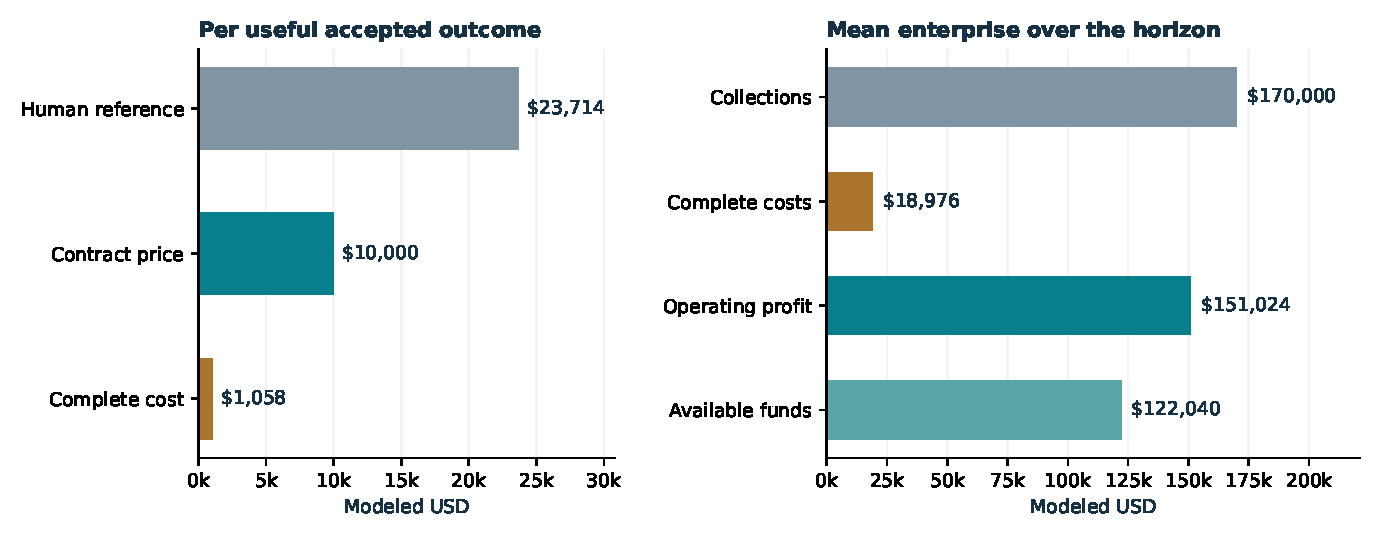
\includegraphics[width=\linewidth]{figures/commercial-core-profile.pdf}
\caption{Commercial core in the reference profile, all values modeled. Left: matched human reference, contract price and fully allocated cost on the same 251 useful outcomes. Right: mean company collections, complete costs, pre-tax-reserve profit and spendable operating funds over 72 business weeks plus runoff. The right panel is per enterprise, not per job.}
\end{figure}

\subsection{Economic and capacity conditions}

The reference profile collects an average of \usd{9,482.07} per useful outcome after defaults and cancellations, rather than treating every quoted \usd{10,000} as collected. Subtracting the full \usd{1,058.40} cost leaves \usd{8,423.67} of complete pre-tax-reserve profit per useful outcome. Holding the observed mix and program fixed, the accounting break-even diagnostic is 1.32 accepted outcomes over the operating horizon, so two such outcomes would clear that static cost threshold. This is not a demand forecast or a survival guarantee: collection timing, lost capacity, quality, reserves and early cash closure still matter.

The cash upper bound and the investment-value bound differ. An average \usd{122,040} is available after modeled costs and reserves in the reference profile, but the existence of funds does not justify an uneconomic candidate. With no demand, all 40 histories close and lose an average \usd{10,148}; preserving the reserve prevents insolvency rather than making the enterprise viable. A different price could change the burdensome profile, but its profitability has not been confirmed under a separately optimized profile-specific policy.

The target configuration uses six workers, each with 24 model-hours and 240 proof-container-hours per week, plus stated aggregate token/request quotas. Mean useful turnaround in the reference profile is 19.16 days and its 95 th percentile is 28 days; initial queue delay is small, but per-worker proof capacity reaches its reservation limit. The weekly fluid schedule cannot establish minute-by-minute burst compliance, arbitrary concurrency or a production service-level guarantee. Reference useful throughput is 0.249 outcomes per enterprise-week; the high-repeat panel tests greater offered demand, not observed customers. Enterprise expansion is outside the optimized control set.

\begin{figure}[ht]\centering
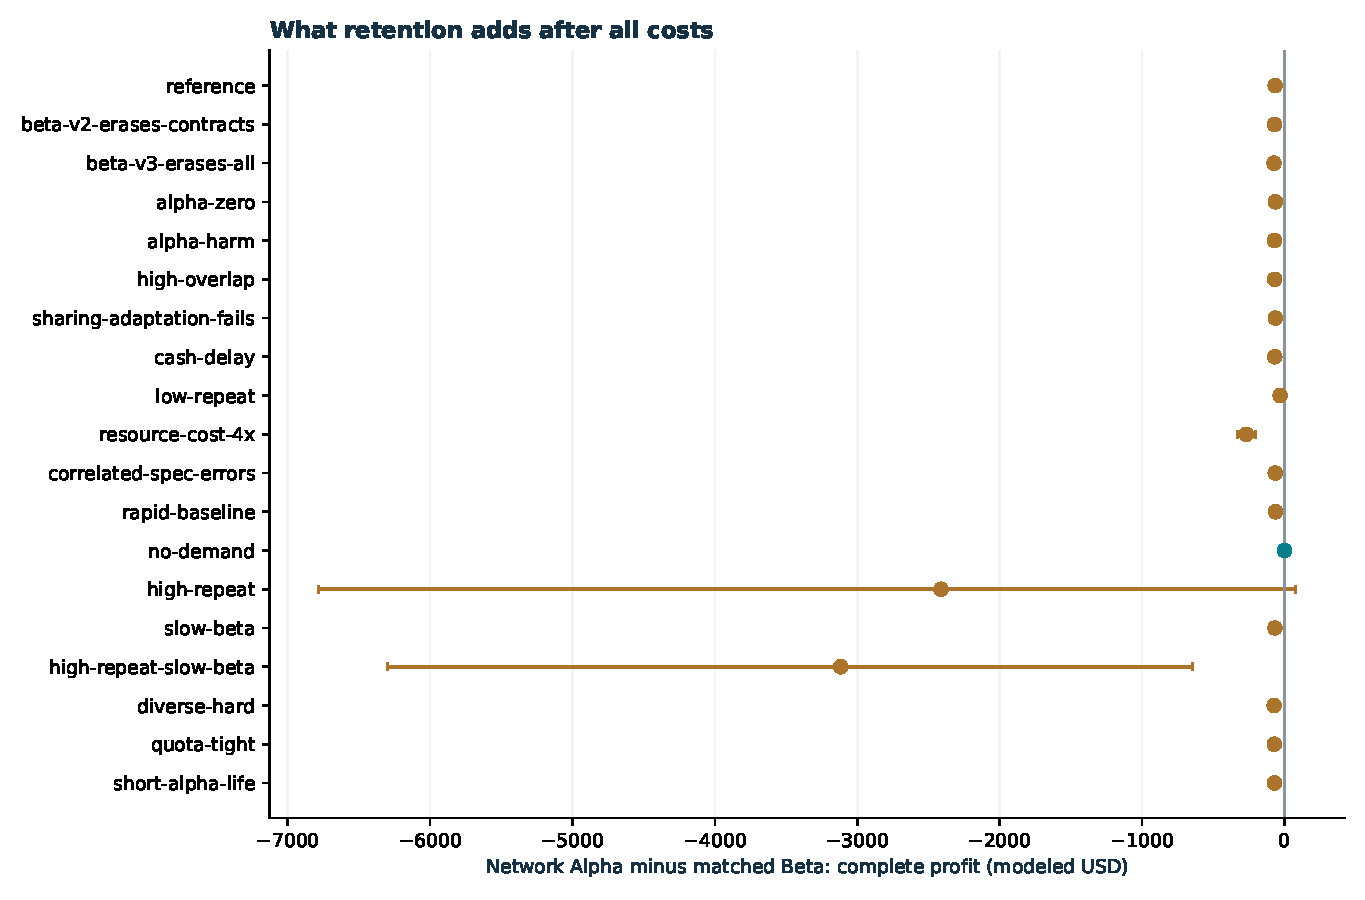
\includegraphics[width=0.93\linewidth]{figures/alpha-conditions.pdf}
\caption{Optional network retention minus matched Beta across every prespecified condition. Intervals are paired-seed bootstrap intervals conditional on the model, not confidence about real-world demand or capability. Negative enhancement value does not erase the separately reported profitable service core.}
\end{figure}

